\section{Compilation et génération du fichier exécutable}

\subsection{Compilation de triangle}
L'exécution du programme triangle permet d'obtenir les instructions en PostScript pour la construction d'un triangle de Pascal de taille de police et de nombre de lignes voulu.
Pour exécuter ce programme il suffit d'exécuter la commande \verb|>./triangle 12 4| ce qui donnera les instructions en PostScirpt pour créer un triangle de Pascal de taille de police 12 et de 4 lignes (code \ref{triangle}).
\begin{lstlisting}[language=PostScript, label=triangle, caption=./triangle 12 4]
newpath 24 245 moveto 38 245 lineto 38 260 lineto stroke newpath 24 245 moveto 24 260 lineto 38 260 lineto stroke /Courier findfont 12 scalefont setfont newpath 25 248 moveto (1) show 
newpath 24 230 moveto 38 230 lineto 38 245 lineto stroke newpath 24 230 moveto 24 245 lineto 38 245 lineto stroke /Courier findfont 12 scalefont setfont newpath 25 233 moveto (1) show 
etc ...
\end{lstlisting}

\subsection{Redirection de la sortie standard}
\label{sec:sortie}

La commande \verb|>./triangle 12 4 > triangle_pascal_12_4.ps| permet de rediriger la sortie standard vers le fichier \verb|triangle_pascal_12_4.ps| qui contient le code PostScript \ref{triangle}.
À l'aide de la commande \verb|> cat triangle_pascal_12_4.ps| on affiche dans le terminal le code PostScript (code \ref{triangle}) enregistré dans \verb|triangle_pascal_12_4.ps|.
À l'aide de la commande \verb|>gv triangle_pascal_12_4.ps| l'interprète de langage PostScript nous permet d'observer la figure \ref{fig:triangle_12_4}.

\begin{figure}[!h]
\begin{centering}
	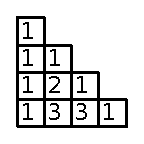
\includegraphics[width=0.5\textwidth]{./images/triangle}
	\caption{Triangle de Pascal de taille de police 12 de 4 lignes.}
	\label{fig:triangle_12_4}
	\end{centering}
\end{figure}

\subsection{Redirection de l'entrée standard}
L'exécution de la commande \verb|> tr "bc" "BC" < Makefile| permet de mettre en majuscule les lettres c et b du fichier \verb|Makefile|. 

\subsection{Tube et chaînage de commandes}
\label{sec:tube}
Lorsque l'on exécute la commande \verb|> date > d| on redirige la sortie de l'exécution de la commande \verb|> date| vers le fichier \verb|d|.
L'exécution de la commande \verb|> tr ":" "_" < d| permet de récupérer ce que contient le fichier \verb|d| afin de remplacer les \verb|:| par des \verb|_|.
À l'aide de l'utilisation d'un tube de redirection il est possible d'effectuer la même manoeuvre sans passer par un fichier intermédiaire et afficher le résultat directement dans le terminal.
C'est ce que permet de faire la commande \verb!date \| tr ":" "_"!.

Ainsi en utilisant les commandes \ref{pipeBash} on obtient la même figure \ref{fig:triangle_12_4} qu'en effectuant les démarche de la section \ref{sec:sortie} qui sera affichée par un interpréteur de PostScript.

\begin{lstlisting}[language=bash, label=pipeBash, caption=Tubes de redirection]
> ./triangle 12 4 | gs -sDEVICE=x11 -q
> ./triangle_12_4 | gv -
\end{lstlisting}













